\documentclass[aspectratio=43,12pt]{beamer}

% Document specific details
\title{Environmental Impact of Housing in England}
\author{Josh Cowley}
\date[May 4th, 2022]{}

\graphicspath{{images/}}

% Document specific packages

%%%%%%%%%%%%%%%%%%%%%%%%%%%%%%%%%%%%%%%%%%%%%%%%%%%%%%%%%%%%%%%%%%%%%%%%%%%%%%%
% IDEALLY MOVE FOLLOWING TO .sty FILE
%%%%%%%%%%%%%%%%%%%%%%%%%%%%%%%%%%%%%%%%%%%%%%%%%%%%%%%%%%%%%%%%%%%%%%%%%%%%%%%

% Persistent packages
\usepackage{hyperref}
\usepackage{bm}
\usepackage{booktabs}
\usepackage{setspace}

% Double-line spacing
\setstretch{1.5}

% Define background images
\newcommand{\bgall}{
    
\includegraphics
        [width=\paperwidth,height=\paperheight]
        {all-page-background}
}

\newcommand{\bgtitle}{
    
\includegraphics
        [width=\paperwidth,height=\paperheight]
        {front-page-background}
}

\makeatletter % Remove in .sty file?



% Apply custom background images based on frame number 
\setbeamertemplate{background canvas}{
    \ifnum\c@framenumber=1%
        % On title page
        \bgtitle
    \else%
        % Other frames background
        \bgall
    \fi%
}

% Custom headline
\setbeamertemplate{headline}{%
    \leavevmode
    \begin{beamercolorbox}[ht=2.5ex,right]{title in head/foot}
    \usebeamerfont{title in head/foot}
        \ifnum\c@framenumber=1%
            \usebeamercolor[fg]{date}%
            \insertshortdate
        \else%
            \href{https://github.com/nclJoshCowley/ANNE-challenge}{github.com/nclJoshCowley/ANNE-challenge}
        \fi%
    \hspace*{1.0 em}
    \end{beamercolorbox}%
}

% Custom footline
\setbeamertemplate{footline}{%
    \leavevmode
    \ifnum\c@framenumber=1%
        % No footline on title page
    \else%
    \begin{beamercolorbox}[ht=2.25ex,dp=1ex,right]{title in head/foot}
        \usebeamerfont{title in head/foot}
        \insertframenumber
        \hspace*{1.0 em}
    \end{beamercolorbox}%
    \fi%
}

% Remove navigation symbols
\setbeamertemplate{navigation symbols}{}

\makeatletter % Remove in .sty file?

% Increase itemize and enumerate spacing
\let\OLDitemize\itemize
\renewcommand\itemize{\OLDitemize\setlength\itemsep{8.0pt plus 2.0pt minus 1.0pt}}

% Convert all title page font colour to be white
\setbeamercolor{title}{fg=white}
\setbeamercolor{author}{fg=white}
\setbeamercolor{institute}{fg=white}
\setbeamercolor{date}{fg=white}

% Section introduction slides (no numbering or footline)
\AtBeginSection[]{
    \begingroup
        \setbeamertemplate{footline}{}
        \begin{frame}[noframenumbering]
            \tableofcontents[currentsection]
        \end{frame}
    \endgroup
}

%%%%%%%%%%%%%%%%%%%%%%%%%%%%%%%%%%%%%%%%%%%%%%%%%%%%%%%%%%%%%%%%%%%%%%%%%%%%%%%
% BEGIN DOCUMENT
%%%%%%%%%%%%%%%%%%%%%%%%%%%%%%%%%%%%%%%%%%%%%%%%%%%%%%%%%%%%%%%%%%%%%%%%%%%%%%%

\begin{document}

\begin{frame}
    \titlepage
\end{frame}

\begin{frame}{Outline}
    \tableofcontents
\end{frame}

\section{Problem Setting}

\begin{frame}{Problem Setting}
    Main objective:
    
    \begin{itemize}
        \item create an environmental indicator for \textbf{housing}.
    \end{itemize}
    
    \vspace{2.0 em}

    We aim to:

    \begin{itemize}
        \item focus on housing efficiency within England;
        \item assess accuracy of EPC ratings as an existing metric;
        \item describe trends in efficiency at a regional level.
    \end{itemize}
\end{frame}

\subsection{EPC? SAP?}

\begin{frame}{EPC? SAP?}
    Home energy efficiency and CO2 emissions assessed by 

    \begin{center}
        \textbf{S}tandard \textbf{A}ssessment \textbf{P}rocedure
    \end{center}

    which is used when awarding

    \begin{center}
        \textbf{E}nergy \textbf{P}erformance \textbf{C}ertificate(s)
    \end{center}

    to homes in the UK.
\end{frame}

\begin{frame}{EPC? SAP?}
    EPC certificates primarily focus on energy efficiency.

    \vspace{1.0 em}

    A SAP rating of 1 - 100 informs the band A - G as shown.

    \begin{figure}[H]
        \centering
        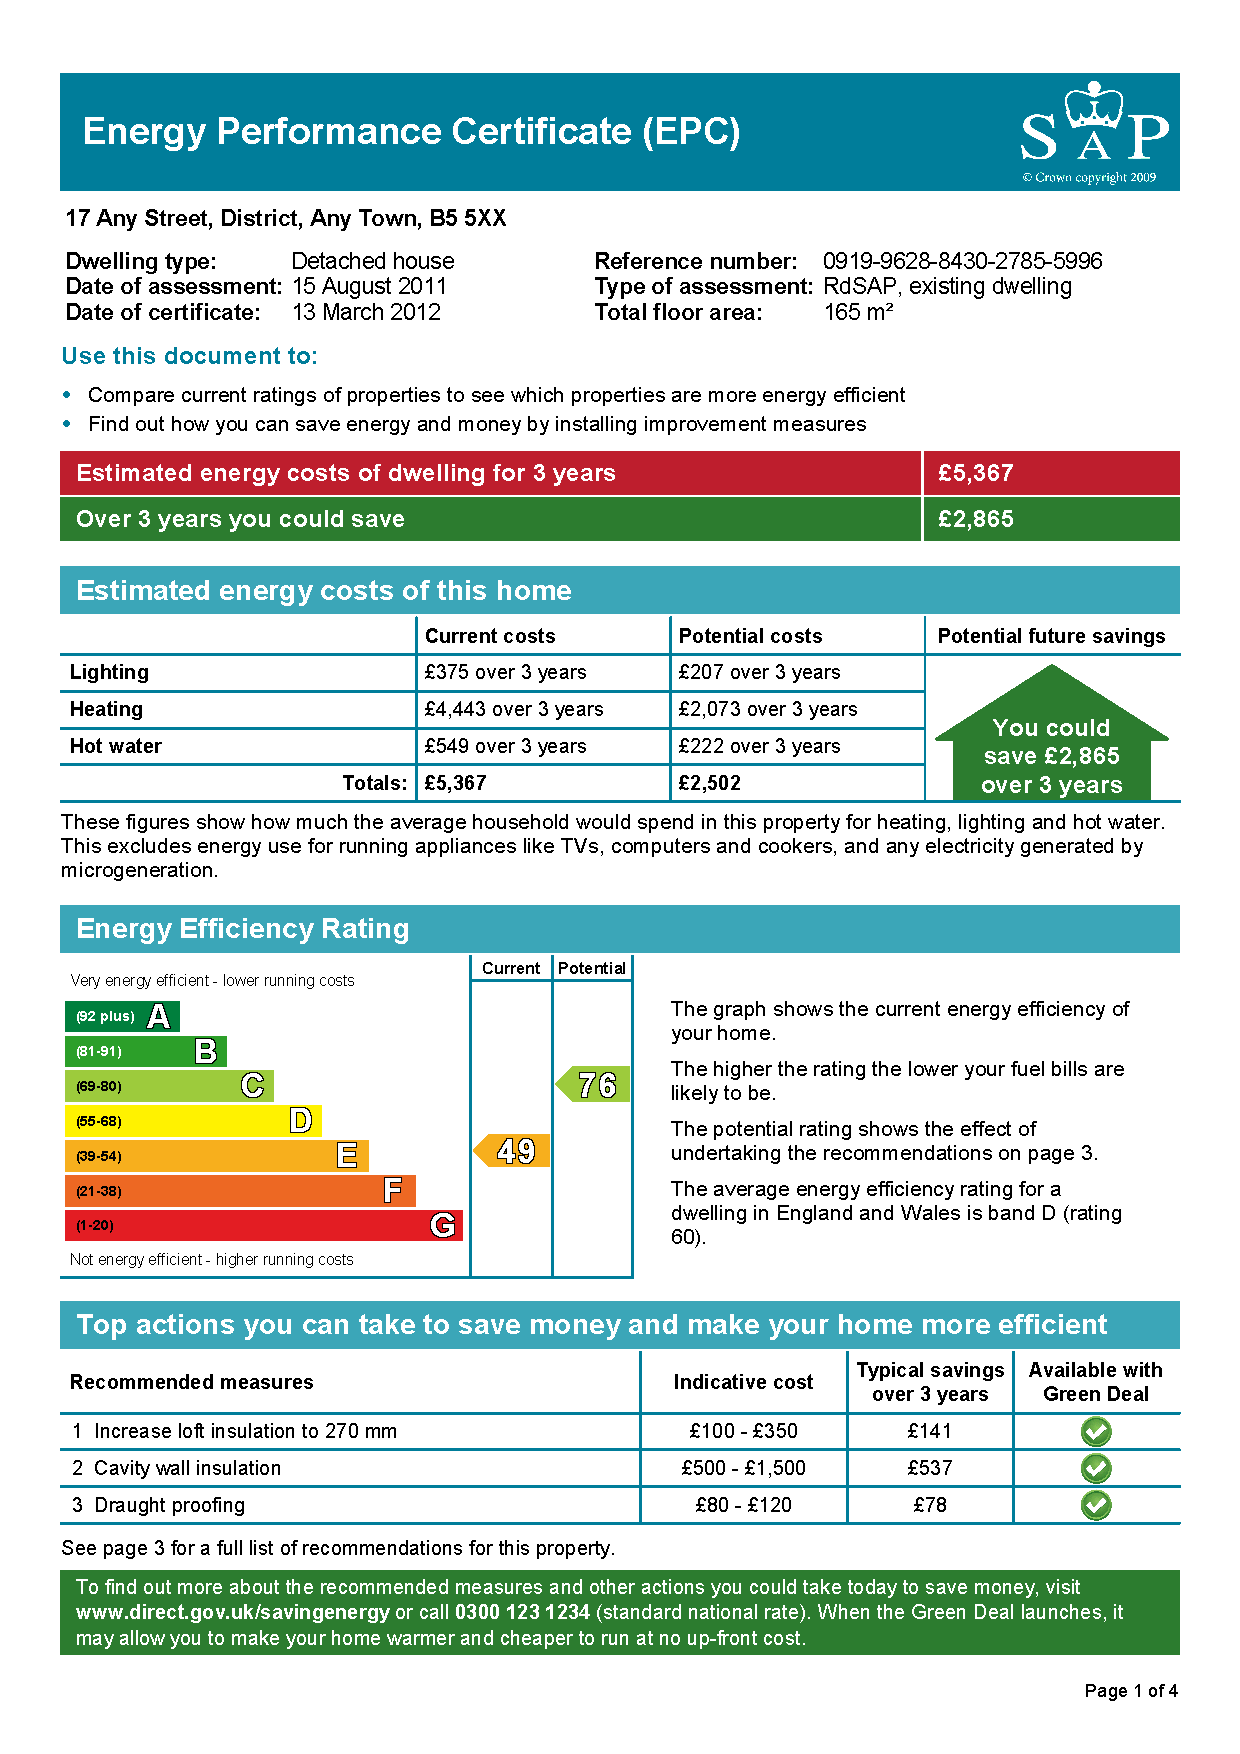
\includegraphics
            [trim = 0cm 8cm 0cm 15cm, clip, page = 1, width = \textwidth]
            {epc-sample-certificate} 
        \caption{Sample EPC certificate (Energy Efficiency Rating).}
        \label{fig:epc-sample-certificate-eer}
    \end{figure}
\end{frame}

\begin{frame}{EPC? SAP?}
    In addition, CO2 emissions highlighted via an environmental impact rating.
    	
    \begin{figure}[H]
        \centering
        \includegraphics
            [trim = 0cm 10.6cm 0cm 15.7cm, clip, page = 4, width = \textwidth]
            {epc-sample-certificate} 
        \caption{Sample EPC certificate (Energy Impact Rating).}
        \label{fig:epc-sample-certificate-eir}
    \end{figure}
\end{frame}

% Source (Information)
% > https://www.gov.uk/guidance/standard-assessment-procedure
% Source (Image)
% > https://assets.publishing.service.gov.uk/government/uploads/system/uploads/attachment_data/file/5996/2116821.pdf

\section{Data}

\subsection{English Housing Survey (EHS)}

\begin{frame}{English Housing Survey (EHS)}
    Annual national survey of two parts commissioned by 
    DLUHC.
    % Department for Levelling Up, Housing and Communities.

    \begin{enumerate}
        \item \textbf{household} interview of occupiers:
        \begin{itemize}
            \item number of occupants;
            \item energy price.
        \end{itemize}

        \pause

        \item physical inspection of the \textbf{dwelling}:
        \begin{itemize}
            \item SAP rating;
            \item boiler type;
            \item double glazing.
        \end{itemize}
    \end{enumerate}
\end{frame}

\begin{frame}{English Housing Survey (EHS)}
    \begin{figure}[H]
        \centering
        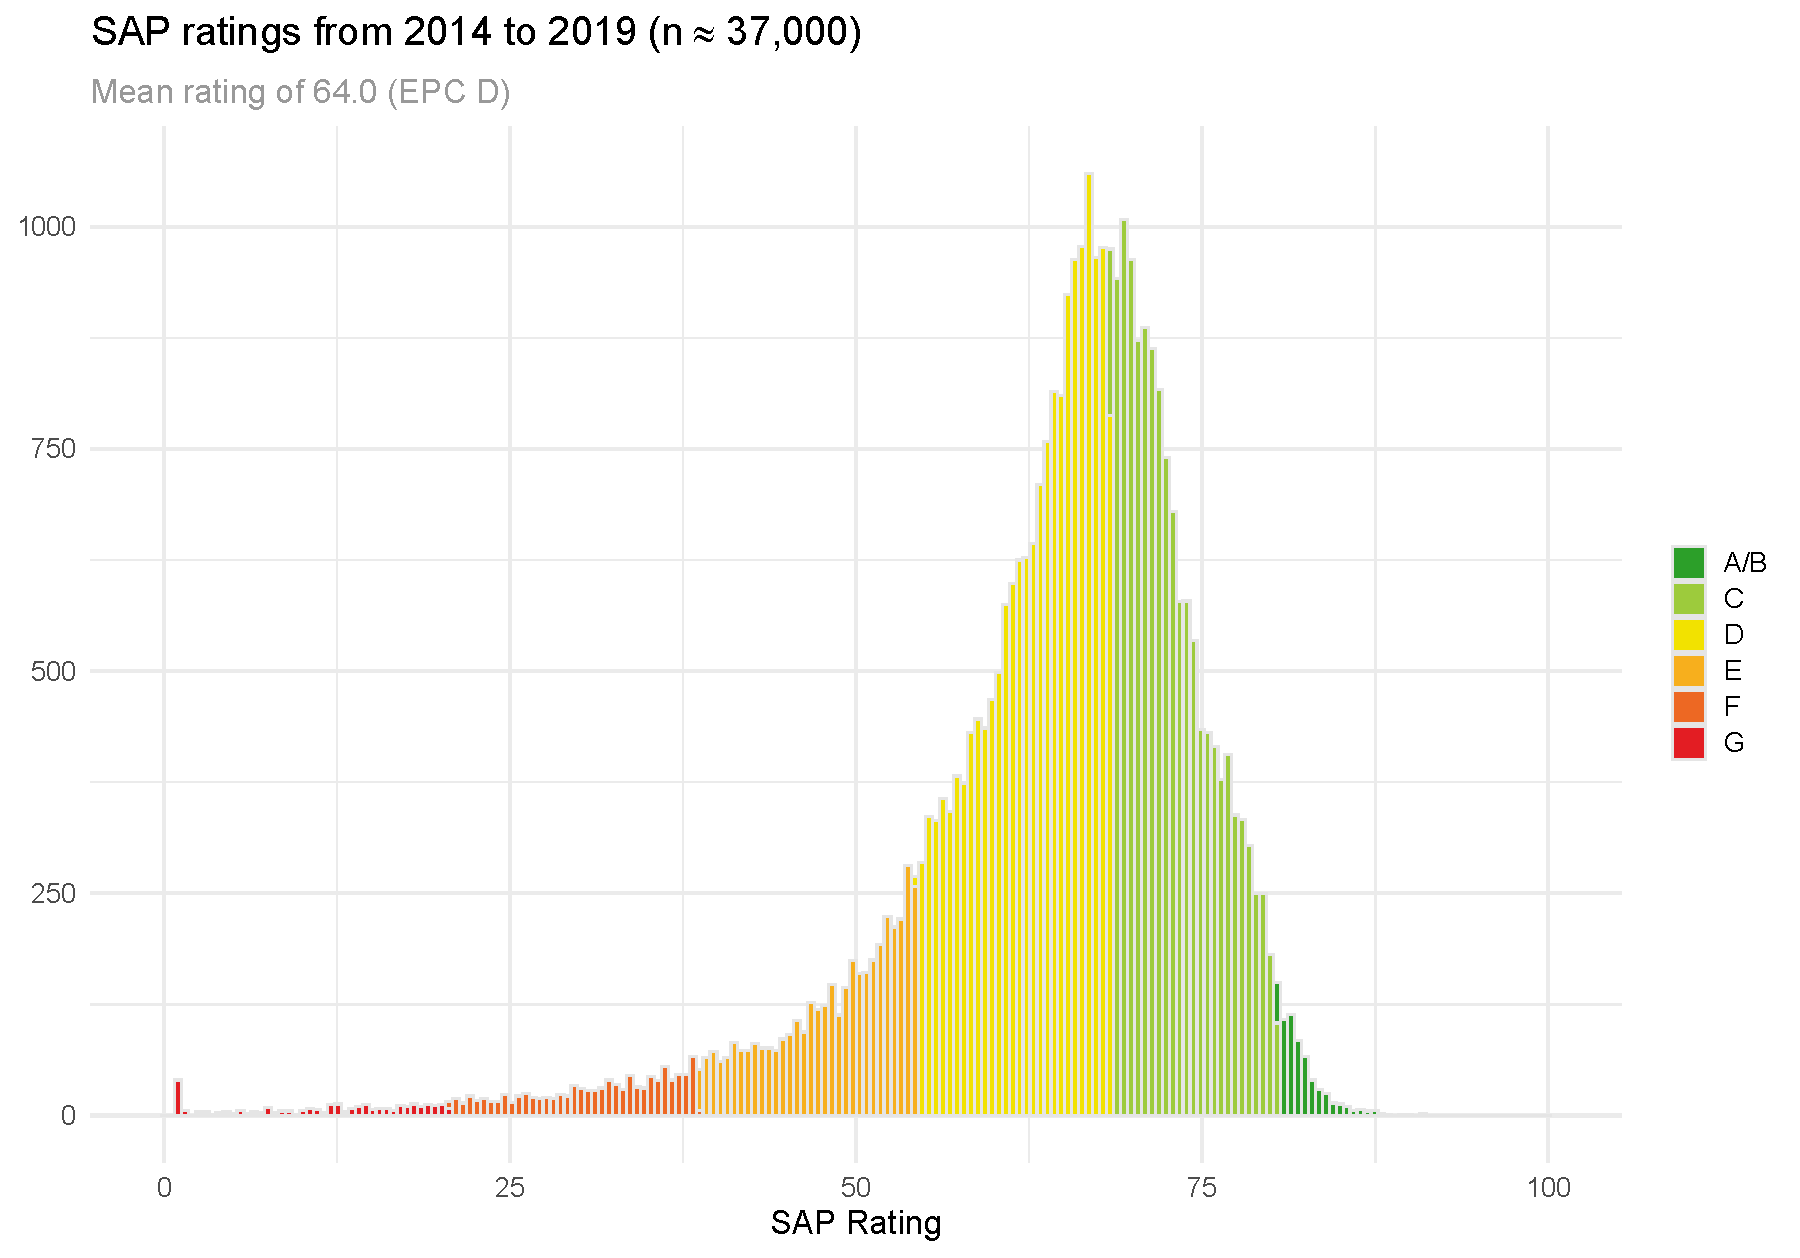
\includegraphics
            [width = \textwidth]
            {fig1_6-1}
        \label{fig:fig1_6-1}
    \end{figure}
\end{frame}
\section{Model A - Multiple Linear Regression}

\subsection{Multiple Linear Regression}

\begin{frame}{Multiple Linear Regression}
    Following data exploration, we ask:

    \vspace{1.0 em}

    \begin{itemize}
        \setlength\itemsep{16.0pt}
        \item Do SAP ratings describe efficiency accurately?
        \item What is (and \textbf{is not}) significant to EPC?
    \end{itemize}

    \vspace{1.0 em}

    Hence, fit a MLR using all relevant features from EHS.
\end{frame}

\begin{frame}{Multiple Linear Regression}
    All features in EHS are \textbf{significant}:

    \begin{itemize}
        \item boiler type;
        \item double glazing;
        \item space heating fuel source;
        \item water heating system;
        \item loft and wall insulation.
    \end{itemize}

    \vspace{0.5 em}

    EHS gives no data on \textbf{renewable technologies}.
\end{frame}
\section{Model B - Multilevel Model}

\subsection{Multilevel Model}

\begin{frame}{Multilevel Model}
    We fit an \textbf{intercept only} model as:

    \begin{equation*}
        \mathrm{SAP}
            = \beta_{\mathrm{Year}}
            + \gamma_{\, \mathrm{Year}, \, \mathrm{Region}}
            + \epsilon
    \end{equation*}

    where
    
    \begin{itemize}
        \item $\beta$ represents a population effect, by year;
        \item $\gamma$ represents a region-specific effect, by year;
        \item $\epsilon$ is a noise term.
    \end{itemize}
\end{frame}

\begin{frame}{Population Effect}
    \begin{figure}[H]
        \centering
        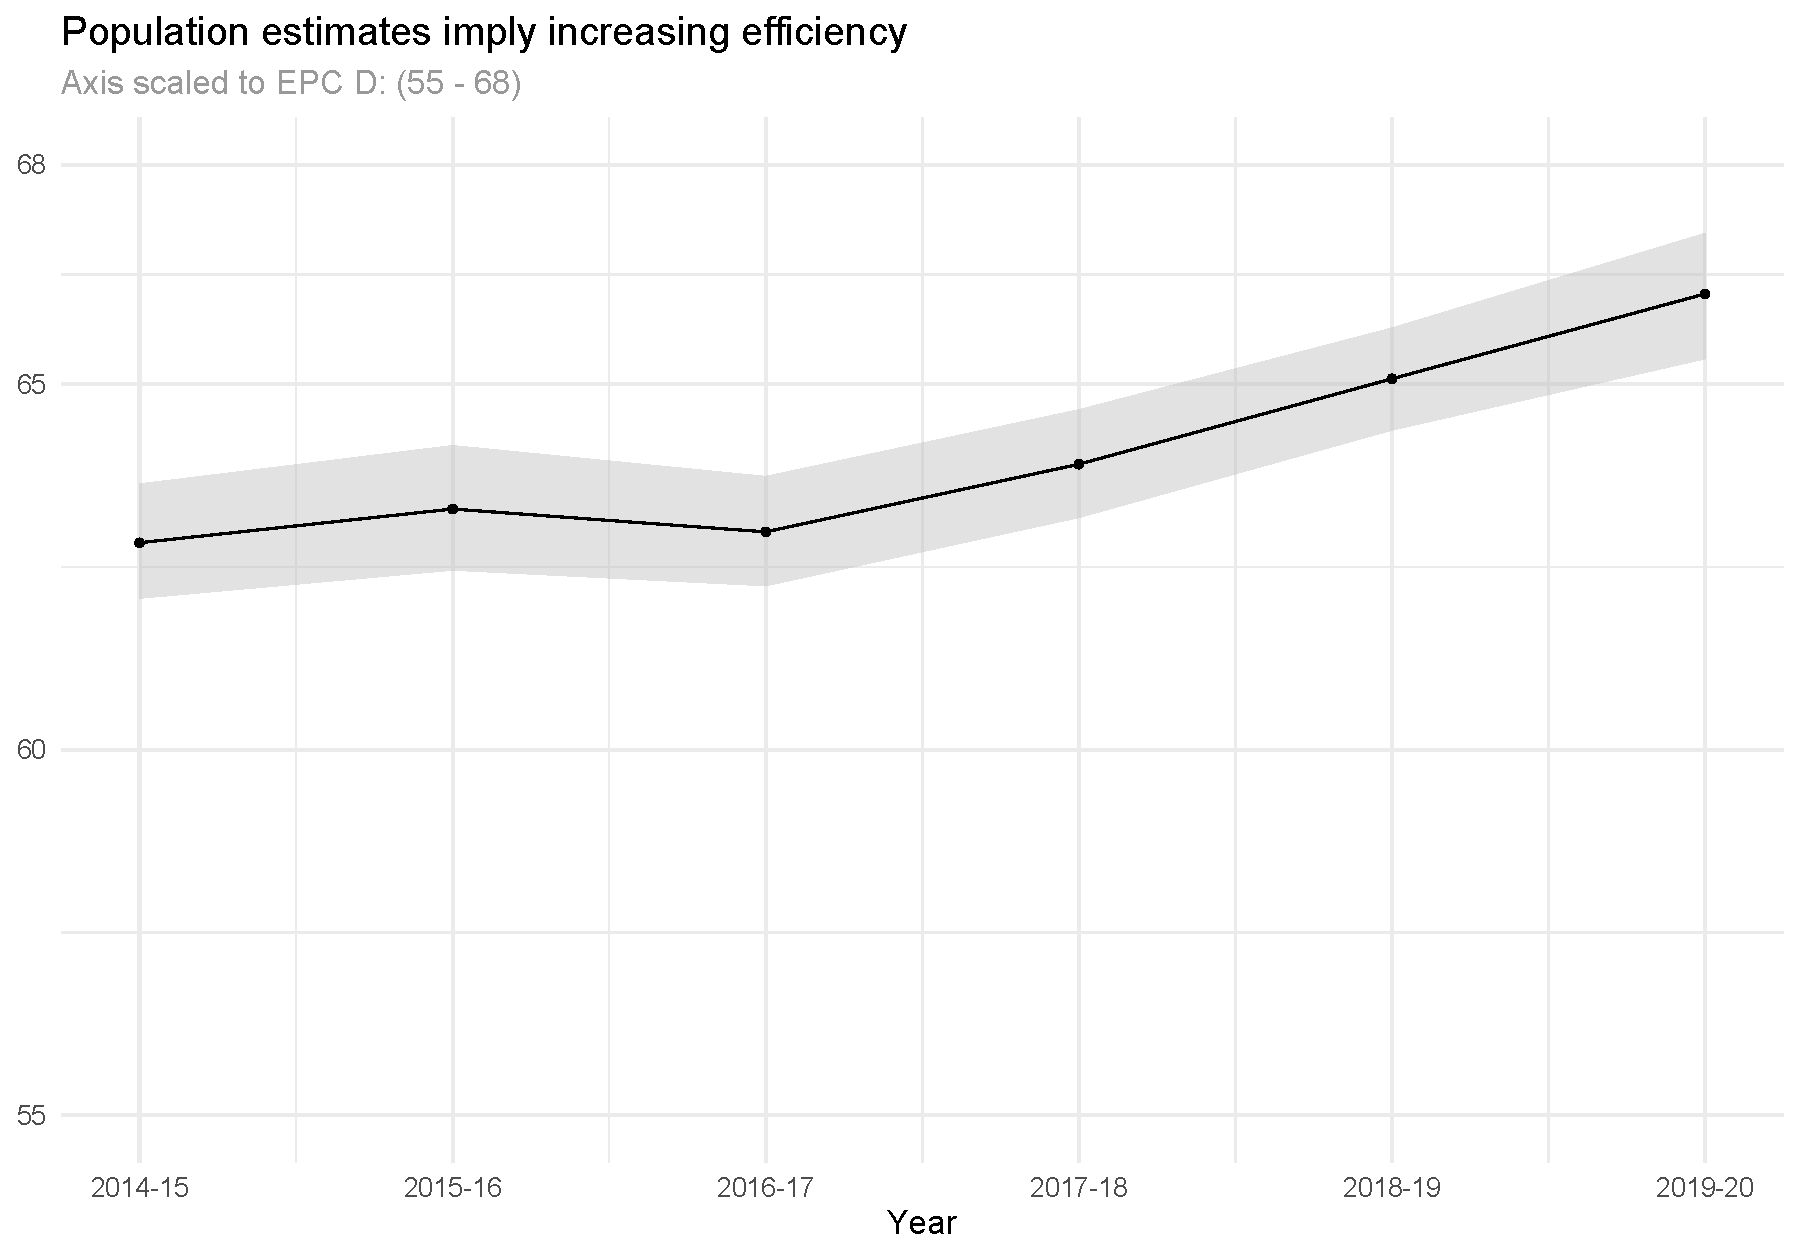
\includegraphics
            [width = \textwidth]
            {fig3_1-1}
        \label{fig:fig3_1-1}
    \end{figure}
\end{frame}

\begin{frame}{Regional Effects}
    \begin{figure}[H]
        \centering
        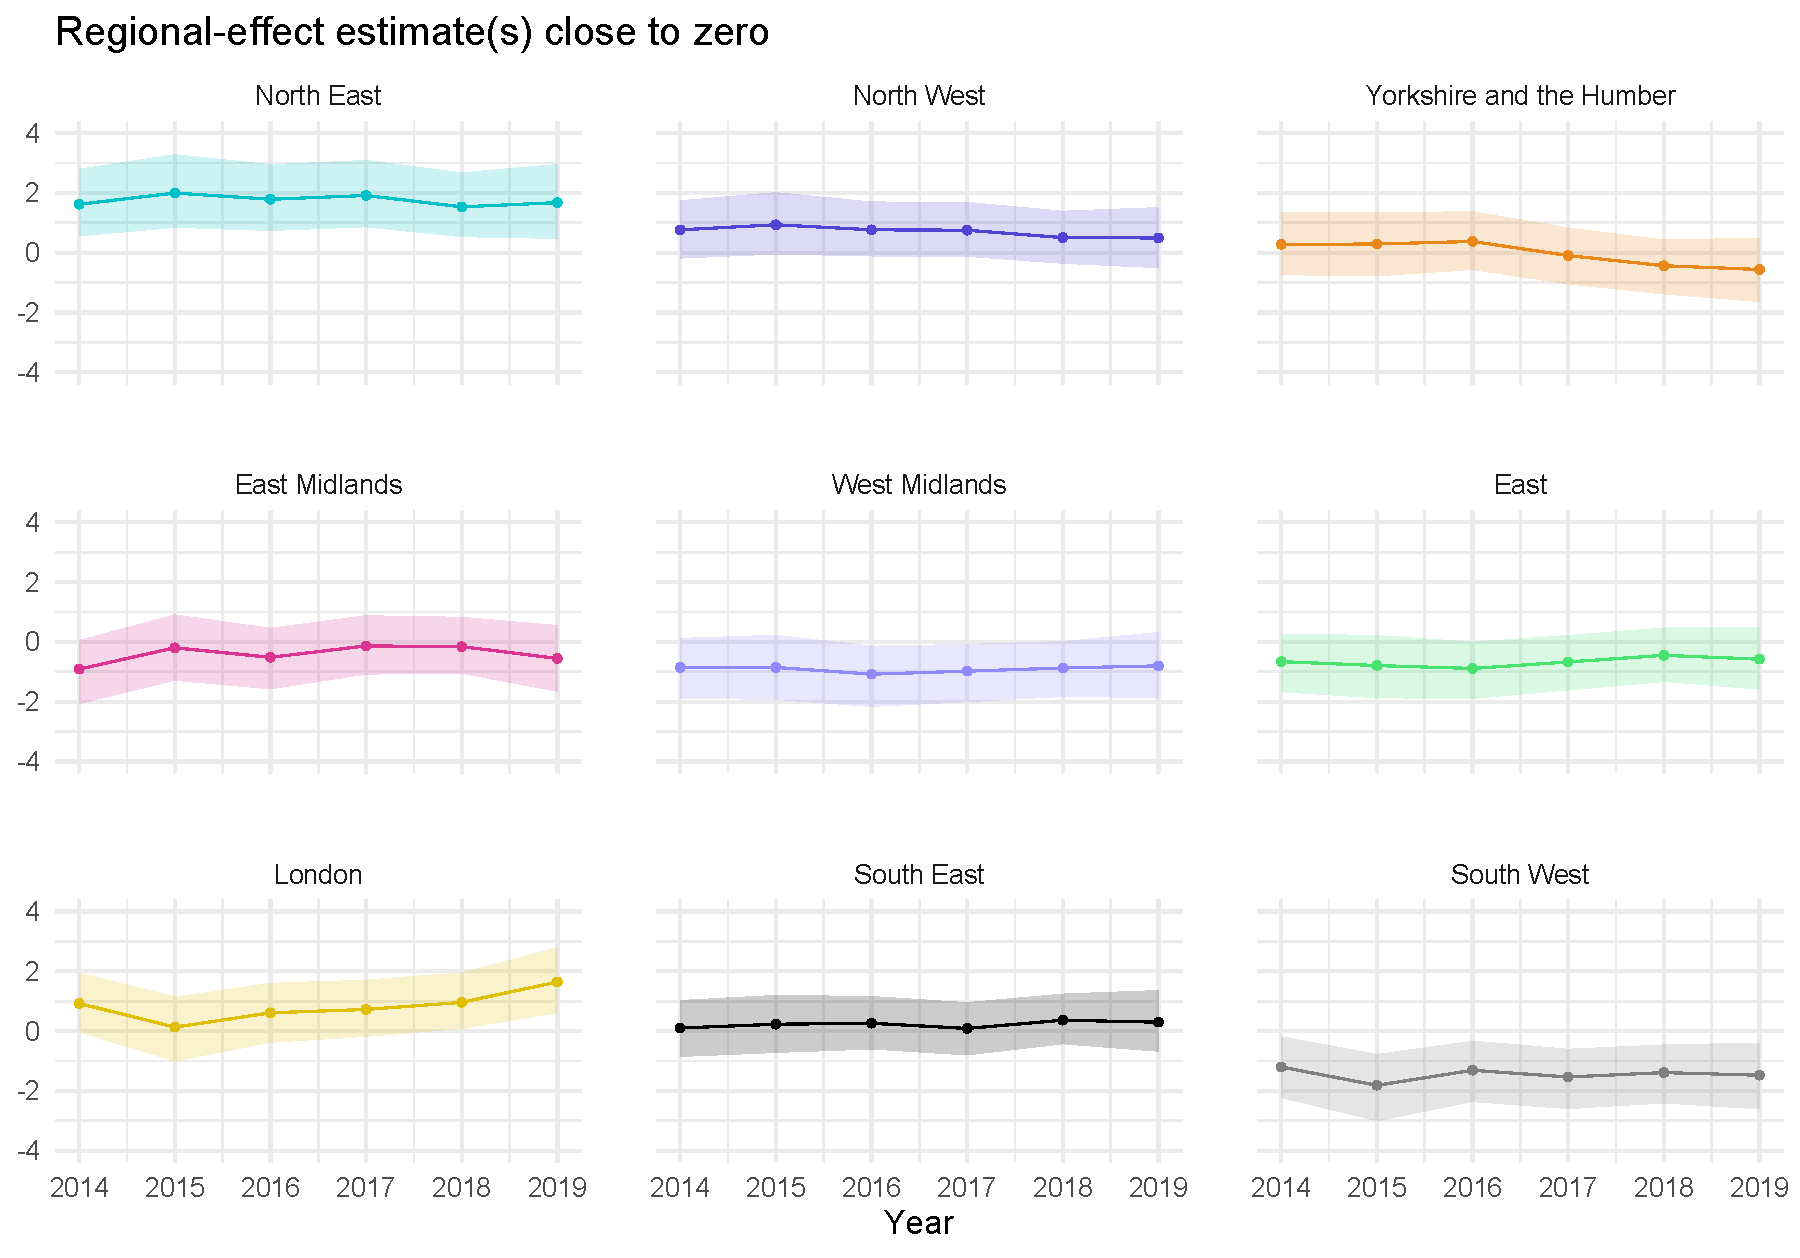
\includegraphics
            [width = \textwidth]
            {fig3_2-1}
        \label{fig:fig3_2-1}
    \end{figure}
\end{frame}

\end{document}